% !TeX root = ../TFG_LaTeX.tex
\section{Transformacions conformes}

\begin{adjustwidth}{1cm}{1cm}

    Les transformacions conformes són un concepte fonamental en l'anàlisi complexa i la seua geometria, amb aplicacions en diversos camps de la ciència i l'enginyeria. Aquestes transformacions tenen la propietat de preservar localment els angles entre corbes que s'intersecten, tant en magnitud com en sentit. En altres paraules, si dues corbes es creuen en un punt formant un cert angle, les seues imatges baix una transformació conforme es creuaran en el punt corresponent formant exactament el mateix angle. Les funcions holomorfes són conformes en tots els punts on la seua derivada és diferent de zero. Per a una exposició detallada i per aprofundir en els conceptes de la teoria de les transformacions conformes, es poden consultar les referències \cite[Cap.3, Secció 2]{ahlfors},\cite[Cap.8]{bruna},\cite[Cap.2]{needham},\cite[Cap.14]{rudin}.

    \begin{subsection}{Corbes i angles en \texorpdfstring{$\mathbb{C}$}{C}}
        
    \begin{definicio}
        Una \textbf{corba} en $\mathbb{C}$ és una aplicació $\gamma:[a,b]\to \mathbb{C}$ contínua. Direm que $\gamma(a)$ és el \textbf{punt inicial} i $\gamma(b)$ el \textbf{punt final}. La imatge de la corba, $\gamma([a,b])\subset \mathbb{C}$ s'anomena \textbf{arc de $\gamma$} i el denotarem per $\gamma*$. Direm que la corba és \textbf{tancada} si $\gamma(a)=\gamma(b)$.
    \end{definicio}    

    \begin{definicio}
        Siga una corba $\gamma:I \to \mathbb{C}, \gamma(t)=x(t)+iy(t)$, on $I\subset R$ és un interval. Direm que $\gamma$ és \textbf{suau} si $x(t), y(t)$ són funcions de classe $\mathcal{C}^1$ i $\gamma'(t)\neq 0 $ per a tot $t$ en $I$. A més, direm que una \textbf{funció} $f:\mathbb{C}\to \mathbb{C}$ és \textbf{suau} si les seues components real i imaginària són de classe $\mathcal{C}^1$.
    \end{definicio}

    Intuïtivament, una corba suau és aquella que no té pics. Veure figura \ref{corba_suau}.

    \begin{figure}[H]
        \centering
        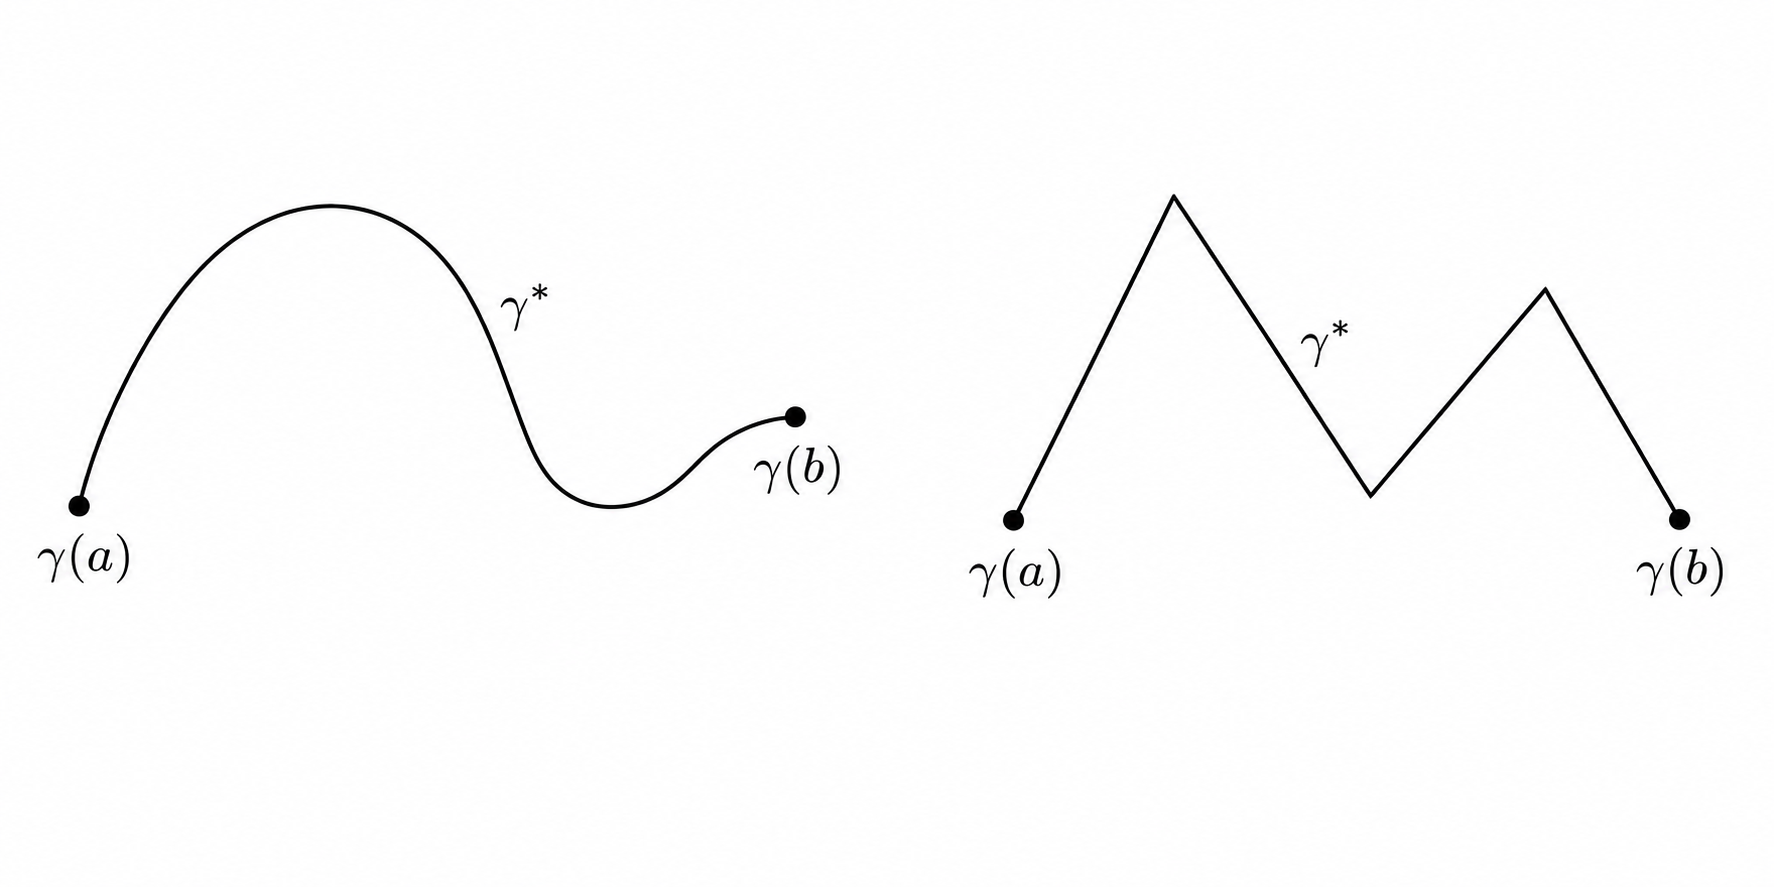
\includegraphics[width=0.5\textwidth]{pictures/corba_suau.png}
        \caption{Corba suau (esquerra) i corba no suau (dreta)}
        \label{corba_suau}
    \end{figure}
    
    \begin{definicio}
        Siga $\gamma:[0,1]\to \mathbb{C}$ una corba suau de la forma $\gamma(t) = x(t) + i y(t)$ i siga $z_0=\gamma(t_0)$, $t_0\in[0,1]$. Si existeix

        \[
            \gamma'(t_0) = \lim_{t \to t_0} \frac{\gamma(t) - \gamma(t_0)}{t-t_0} = x'(t_0) + i y'(t_0),
        \]
        i $\gamma'(t_0)\neq 0$, definim $\gamma'(t_0)$
        com el \textbf{vector tangent} a la corba $\gamma$ en $z_0$. 

    \end{definicio}
    
    \begin{definicio}
        
        Donades dues corbes suaus $\gamma_1,\gamma_2:[0,1]\to\mathbb{C}$ de manera que $\gamma_1(t_1)=\gamma_2(t_2)=z_0$ per a $t_1,t_2\in[0,1]$ i suposant que $\gamma'_1(t_1),\gamma'_2(t_2)\neq 0$, definim l'\textbf{angle entre $\gamma_1$ i $\gamma_2$ en $z_0$}  com
        \[
            arg\left( \frac{\gamma'_2(t_2)}{\gamma'_1(t_1)} \right)=\arg \gamma_2'(t_2)-\arg \gamma_1'(t_1),
        \]
        entenent-ho com a mòdul $2\pi$, és a dir, que 2 angles que difereixen en un múltiple de $2\pi$ se consideren el mateix.

    \end{definicio}

    És important tindre en compte que l'angle és orientat, i per tant és important mantindre l'ordre al calcular la diferència dels arguments.


    \begin{exemple}
        Si tenim les dues corbes suaus
        \[
            \begin{aligned}
            \gamma_1:[0,1] \to \mathbb{C}, \quad \gamma_1(t) &= t + i t^2 \\
            \gamma_2:[0,1] \to \mathbb{C}, \quad \gamma_2(t) &= t + i\sin(t)
            \end{aligned}
        \]
        aleshores $\gamma_1(0)=\gamma_2(0)=0$ i  els seus vectors tangents en el 0 són, respectivament, 
        \[
            \begin{aligned}
            \gamma'_1(0) &= 1 \\
            \gamma'_2(0) &= 1+i
            \end{aligned}
        \]
        i per tant, l'angle entre les dues corbes en el 0 és 
        \[
            arg(1+i)-arg(1)=arg(1+i)=\frac{\pi}{4}
        \] 

    \end{exemple}

    \begin{figure}[H]
        \centering
        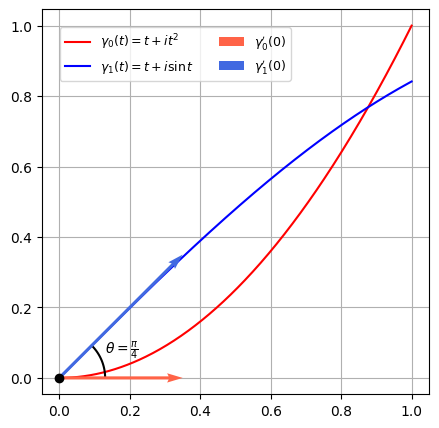
\includegraphics[width=0.5\textwidth]{pictures/angle_entre_dos_corbes.png}
        \caption{Angle entre $\gamma_1$ i $\gamma_2$ en el punt 0.}
        \label{angle_entre_dos_corbes}
    \end{figure}

    \begin{teorema}
        Siga $\gamma:[0,1]\to \mathbb{C}$ una corba suau de la forma $\gamma(t) = x(t) + i y(t)$ amb $z_0=\gamma(t_0)$, sent $t_0\in[0,1]$. Si $f:U\to \mathbb{C}$ és holomorfa en $z_0\in U$, aleshores $f(\gamma(t))$ és una corba tal que el seu vector tangent en $f(z_0)$ ve donat per
        \begin{equation}
            (f \circ \gamma)'(t_0)=f'(z_0)\gamma'(t_0).
            \label{eq1rc}
        \end{equation}
        \label{teo_expressio_vect_tang_imatge}
    \end{teorema}

    \begin{proof}
        Primer es considera el cas $\gamma'(t_0) \neq 0$. Es té que $\gamma(t) = \gamma(t_0)$ per a $t$ a prop de $t_0$, $t \neq t_0$, i es pot escriure
        \[
            \frac{f(\gamma(t))-f(\gamma(t_0))}{t-t_0} = \frac{f(\gamma(t))-f(\gamma(t_0))}{\gamma(t)-\gamma(t_0)} \frac{\gamma(t)-\gamma(t_0)}{t-t_0}
        \]
        i al prendre límits, com $f$ és analítica en $z_0$ s'obté l'expressió (\ref{eq1rc}).

        Si pel contrari $\gamma'(t_0) = 0$, aleshores com $f(z)$ és diferenciable en $z_0$, el quocient en diferències $(f(z)-f(z_0)/(z-z_0))$ està afitat prop de $z_0$, és a dir, si $\varepsilon >0$,
        \[
            \left|\frac{f(z)-f(z_0)}{z-z_0}\right| \leq C
        \]
        per a alguna constant real $C$ i per a tot $z$ tal que $0 < |z-z_0| < \varepsilon$. 

        Per tant, $|f(\gamma(t))-f(\gamma(t_0))| \leq C |\gamma(t)-\gamma(t_0)|$ per a $z$ a prop de $z_0$ i, conseqüentment,
        \[
            \left|\frac{f(\gamma(t))-f(\gamma(0))}{t}\right| \leq C \left|\frac{\gamma(t)-\gamma(0)}{t}\right|.
        \]
        Com la part de la dreta tendeix a $t_0$ quan $t$ tendeix a $0$, es té que $(f \circ \gamma)'(t_0) = 0$.

        Així, en aquest cas la igualtat es certa perquè $(f \circ \gamma)'(t_0) = 0 = f'(\gamma(t_0))\gamma'(t_0)$.
    \end{proof}

    \begin{nota}
        Es pot pensar el vector tangent com un vector en el pla amb origen en $z_0$. El teorema anterior desprén que, en realitat, compondre una corba parametritzada amb $f(z)$ té l'efecte sobre el vector tangent $\gamma'(t_0)$ de multiplicar-lo per $f'(z_0)$ i traslladar l'origen a $w_0 = f(z_0)$.

        Si el vector tangent està representat per $z - z_0 = \gamma'(t_0)$, aleshores el vector tangent a la corba imatge està representat per $w - f(z_0) = f'(z_0)(z - z_0)$.

        Pel que fa al vector tangent en $z_0$, l'efecte de compondre amb $f(z)$ és el mateix que el d'utilitzar la funció lineal
        \[
        f(z_0) + f'(z_0)(z - z_0),
        \]
        que és l'aproximació de Taylor de primer ordre de $f(z)$ en $z_0$.

        Com el residu d'aquesta aproximació de Taylor, $R(z)$ satisfà
        \[
        \frac{R(z)}{z - z_0} \to 0 \quad \text{quan } z \to z_0,
        \]
        tenim que $R(z)$ no té cap efecte sobre els vectors tangents.
    \end{nota}

    \end{subsection}

    \begin{subsection}{Transformacions conformes}

    A continuació introduïm el concepte de funció conforme, que, com ja hem comentat a la introducció d'aquest capítol, intuïtivament és aquella que preserva angles. Veure figura \ref{apl_conf1}.

    \begin{definicio}
        Siga $f:U\subset \mathbb{C}\to \mathbb{C}$ una funció complexa, i siga $z_0\in U$. Direm que $f$ és \textbf{conforme en} $z_0$ si per a qualsevol dues corbes $\gamma_1,\gamma_2:[0,1]\to \mathbb{C}$ tals que $\gamma_1(t_1)=\gamma_2(t_2)=z_0$, on $t_1,t_2\in[0,1]$, i amb vectors tangents en $z_0$ no nuls, les corbes $f \circ \gamma_1$ i $f \circ \gamma_2$ tenen tangents no nul·les en $f(z_0)$ i l'angle entre $(f \circ \gamma_1)'(z_0)$ i $(f \circ \gamma_2)'(z_0)$ és el mateix que l'angle entre $\gamma_1'(z_0)$ i $\gamma_2'(z_0)$, és a dir, que 
        \[
            \operatorname{arg}\left(\frac{(f\circ\gamma_1)'(t_1)}{(f\circ\gamma_2)'(t_2)}\right)=\operatorname{arg}\left(\frac{\gamma_1'(t_1)}{\gamma_2'(t_2)}\right).
        \]

    \end{definicio}

    \begin{figure}[H]
        \centering
        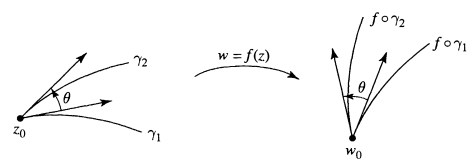
\includegraphics{pictures/Aplicacio_conforme.png}
        \caption{$f$ preserva angles.}
        \label{apl_conf1}
    \end{figure}

    \begin{exemples}
        \leavevmode
        \begin{itemize}
            \item Les dilatacions $f(z)=az$, $a$ en $\mathbb{C}\backslash \{0\}$, i les translacions $f(z)=z+b$, $b$ en $\mathbb{C}$ evidentment conserven angles, i per tant són conformes en qualsevol punt.
            \item La funció conjugat $f(z)=\overline{z}$ no és conforme perquè com $f(z)$ inverteix l'orientació, l'angle entre dues corbes que passen per $z_0$ i l'angle entre les seues imatges tindrà l'orientació invertida, tot i que el seu mòdul siga el mateix.
        \end{itemize}
    \end{exemples}

    \begin{teorema}
        Si $f:\mathbb{C}\to \mathbb{C}$ és holomorfa en $z_0$ i $f'(z_0) \neq 0$, aleshores $f(z)$ és conforme en $z_0$.
        \label{teo_holo_imp_conf}
    \end{teorema}

    \begin{proof}
        Si $\gamma_1$ i $\gamma_2$ són dues corbes i $z_0 = \gamma_1(t_1) = \gamma_2(t_2)$, on $t_1,t_2\in[0,1]$, amb vectors tangents en $z_0$ no nuls, pel Teorema \ref{teo_expressio_vect_tang_imatge}, sabem que les tangents a les corbes $f \circ \gamma_1$ i $f \circ \gamma_2$ s'obtenen multiplicant les respectives tangents a $\gamma_1$ i a $\gamma_2$, és a dir, $\gamma_1'(t_1)$ i $\gamma_2'(t_2)$, per $f'(z_0)$.

        Aleshores els arguments d'ambdues tangents es veuen augmentats pel mateix angle, és a dir, per l'argument de $f'(z_0)$, que és un nombre complex amb mòdul distint de $0$. Per tant, l'angle entre les corbes no canvia.
    \end{proof}

    

    És també cert el recíproc:

    \begin{teorema}
         Siga $g:U\subset \mathbb{C}\to \mathbb{C}$. Si $g$ és conforme en $z_0\in U$, i la corresponent $g:U\subset\mathbb{R}^2\to\mathbb{R}^2$ és de classe $\mathcal{C}^1$ amb $J_g(z_0)\neq 0$, aleshores $g$ és derivable en $z_0$ i $g'(z_0)\neq 0$.
        \label{teo_conf_imp_holo}
    \end{teorema}

    \begin{proof}
        Siga $\gamma(t)=z_0+te^{i\theta}$, on $t\in[-\varepsilon,\varepsilon]$, $\varepsilon>0$, i on $\theta$ fixe, és a dir, estem prenent un segment fixe que passa per $z_0$ amb vector tangent $\gamma'(t)=e^{i\theta}=(cos(\theta),sin(\theta))$.
        
        A més, siguen $u(x,y),v(x,y)$ les components de $g$, és a dir, que $g(x+iy)=u(x,y)+iy(x,y)$, i denotem $z_0=x_0+iy_0$, de forma que quan, més endavant en la demostració, parlem d'una funció en $\mathbb{R}^2$ avaluada en $z$ o en $z_0$, en realitat estem parlant d'avaluar-la en $(x,y)$ o en $(x_0,y_0)$, respectivament.
        
        Considerem $g\circ\gamma$. Com $g$ és de classe $\mathcal{C}^1$, es té que per la Regla de la Cadena (Teorema \ref{reglacadena}),
        \[
            d(g\circ\gamma(t))_{t=0}=dg_{\gamma(0)}\gamma'(0)=dg_{\gamma(0)}(cos(\theta),sin(\theta))
        \]

        Ara bé, com
        \[
            dg_{z_0}=\left.\begin{pmatrix}
                D_1u & D_2u\\
                D_1v & D_2v
            \end{pmatrix}(x,y)\right|_{(x,y)=(x_0,y_0)},
        \] 
        aleshores ens queda, identificant $\mathbb{R}^2$ amb $\mathbb{C}$, que 
        \[
            d(g\circ\gamma(t))_{t=0}=
            \left.\begin{pmatrix}
                D_1u & D_2u\\
                D_1v & D_2v
            \end{pmatrix}(x,y)\right|_{(x,y)=(x_0,y_0)}
            \begin{pmatrix}
                cos(\theta)\\
                sin(\theta)
            \end{pmatrix}=
        \]
        \[
            ((D_1u cos(\theta) + D_2u sen(\theta)) + i(D_1v cos(\theta) + D_2v sen(\theta)))_{z_0}=
        \]
        \[
            (D_1u+iD_1v)cos(\theta)+(D_2u+iD_2v)sin(\theta)_{z_0}.
        \]
        Ara bé, com $e^{i\theta}=cos(\theta)+isin(\theta)$ i $e^{i\theta}=cos(\theta)-isin(\theta)$ això ara ho podem reescriure com
        \[
            \left[e^{i\theta}\left(\frac{D_1u-iD_2u+D_2v+iD_1v}{2}\right)+e^{-i\theta}\left(\frac{D_1u-D_2v+i(D_1v+D_2u)}{2}\right)\right]_{z_0}
        \]
        En el primer parèntesis el que tenim és $\frac{\partial g}{\partial z}=\frac{1}{2}(\frac{\partial g}{\partial x}-i \frac{\partial g}{\partial y})$, i en el segon tenim $\frac{\partial g}{\partial \overline{z}}=\frac{1}{2}(\frac{\partial g}{\partial x}+i \frac{\partial g}{\partial y})$. Per tant, ens queda que
        \[
            (g\circ\gamma)'(t)=e^{i\theta}\frac{\partial g}{\partial z}(z_0)+e^{-i\theta}\frac{\partial g}{\partial \overline{z}}(z_0).
        \]
        Ara bé, com $g$ és conforme en $z_0$, conserva els angles. Aleshores per a tot parell de corbes $\gamma_1,\gamma_2$ tals que $\gamma_1(t_1)=\gamma_2(t_2)=z_0$, on $t_1,t_2\in[0,1]$, es té que 
        \[
            \operatorname{arg}\left(\frac{(g\circ\gamma_1)'(t_1)}{(g\circ\gamma_2)'(t_2)}\right)=\operatorname{arg}\left(\frac{\gamma_1'(t_1)}{\gamma_2'(t_2)}\right).
        \]
        D'aquesta forma, 
        \[
            \operatorname{arg}((g\circ\gamma_1)'(t_1))-\operatorname{arg}((g\circ\gamma_2)'(t_2))=\operatorname{arg}(\gamma_1'(t_1))-\operatorname{arg}(\gamma_2'(t_2)).
        \]
        Reordenant,
        \[
            \operatorname{arg}((g\circ\gamma_1)'(t_1))-\operatorname{arg}(\gamma_1'(t_1))=\operatorname{arg}((g\circ\gamma_2)'(t_2))-\operatorname{arg}(\gamma_2'(t_2)).
        \]
        Per tant, 
        \[
            \operatorname{arg}\left(\frac{(g\circ\gamma_1)'(t_1)}{\gamma_1'(t_1)}\right)=\operatorname{arg}\left(\frac{(g\circ\gamma_2)'(t_2)}{\gamma_2'(t_2)}\right).
        \]
        Això vol dir que $\operatorname{arg}\left(\frac{(g\circ\gamma)'(0)}{\gamma'(0)}\right)$ no depén de $\theta$. Per tant, 
        \[
            \operatorname{arg}\left(\frac{e^{i\theta}\frac{\partial g}{\partial z}+e^{-i\theta}\frac{\partial g}{\partial \overline{z}}}{e^{i\theta}}\right)_{z_0}=\operatorname{arg}\left(\frac{\partial g}{\partial z}+e^{-2i\theta}\frac{\partial g}{\partial \overline{z}}\right)_{z_0}.
        \]
        Aleshores tenim que $\frac{\partial g}{\partial \overline{z}}(z_0)=\frac{1}{2}(\frac{\partial g}{\partial x}(z_0)+i \frac{\partial g}{\partial y}(z_0))=0$, i conseqüentment $\frac{\partial g}{\partial x}(z_0)=-i \frac{\partial g}{\partial y}(z_0)$. Però com $g(x + iy) = u(x, y)+iv(x, y)$, això és el mateix que dir que
        \begin{equation*}
            \begin{aligned}
                \frac{\partial u}{\partial x}(z_0) &= \frac{\partial v}{\partial y}(z_0), \\
                \frac{\partial u}{\partial y}(z_0) &= -\frac{\partial v}{\partial x}(z_0).
            \end{aligned}
        \end{equation*}
        Però aquestes equacions són exactament les equacions de Cauchy-Riemman (Teorema \ref{cauchy_riemann}). Per tant, $g$ és holomorfa en $z_0$, i a més, com per hipòtesi $0\neq |J_g(z_0)|=|g'(z_0)|$, tenim que $g'(z_0)\neq 0$.

    \end{proof}

    Podem combinar els Teoremes \ref{teo_holo_imp_conf} i \ref{teo_conf_imp_holo} per a obtindre el següent resultat.

    \begin{corolari}
        Si $f:U\subset\mathbb{C}\to \mathbb{C}$ és una funció complexa i $f'(z_0)\neq 0$ per a $z_0\in U$, tenim que $f$ és derivable en $z_0$ si i només si $f$ és conforme.
        \label{nota_conf_sii_holomorfa}
    \end{corolari}

    \begin{definicio}
        Considerem una bijecció $g:U\to V$ entre oberts de $\mathbb{C}$ que és conforme a cada punt de $U$. Si entesa com a funció de $\mathbb{R}^2$ en $\mathbb{R}^2$, $g$ és de classe $\mathcal{C}^1$ i té jacobià $J_g(z)\neq 0$ per a tot $z\in U$ direm que $g$ és una \textbf{transformació conforme}.
    \end{definicio}

    \begin{corolari}
        Si $U,V$ són oberts de $\mathbb{C}$, tenim que $g:U\subset \mathbb{C}\to V$ és una transformació conforme si i només si $g$ és holomorfa i bijectiva.
        \label{tc_sii_holo_i_bij}
    \end{corolari}

    \begin{proof}
        Si $g:U\to V$ és una transformació conforme, aleshores per definició ja és bijectiva, i a més com és conforme en cada punt d'$U$. Tenim també per definició que $g$, entesa com a funció de $\mathbb{R}^2$ en $\mathbb{R}^2$, és de classe $\mathcal{C}^1$ i té jacobià $J_g(z)\neq 0$ en tot punt d'$U$. Així, podem aplicar el Teorema \ref{teo_conf_imp_holo} i afirmar que és holomorfa en tot punt d'$U$.

        Recíprocament, suposem que $g:U\to V$ és una bijecció holomorfa. En particular és injectiva, i com $U$ és un obert, aleshores, entesa com a funció de $\mathbb{R}^2$ en $\mathbb{R}^2$, és de classe $\mathcal{C}^1$ i té jacobià $J_g(z)\neq 0$ en tot punt d'$U$. Això es tradueix en variable complexa com que $g'(z)\neq 0$ per a tot $z\in U$. Així, pel Teorema \ref{teo_holo_imp_conf}, es té que $g$ és conforme en tot $U$, i per tant és una transformació conforme.
    \end{proof}

    Com que les aplicacions conformes conserven angles, es pot afirmar que les transformacions conformes converteixen corbes ortogonals, és a dir, aquelles que es tallen formant un angle recte, en corbes també ortogonals, així com famílies de corbes ortogonals en famílies d'aquest mateix tipus. 

    \begin{exemple}
        La funció $f(z)=e^z$, que és holomorfa en tot $\mathbb{C}$ i la seua derivada no s'anul·la per a cap $z$, transforma la malla ortogonal formada per les línies verticals i horitzontals en altra malla ortogonal formada per circumferències concèntriques com a imatge de les rectes verticals, i rajos que s'emanen des de l'origen (sense incloure'l) com a imatge de les rectes horitzontals.
    \end{exemple}

    Una cosa molt semblant passa per a qualsevol funció holomorfa i no constant $f = u+iv$ en un conjunt obert i connex $U$. Primerament, es fixa un punt $z_0$ on $f'(z_0) \neq 0$, i es consideren les dues corbes $A:=\{u(z)=u(z_0)\}$ i $B:=\{v(z)=v(z_0)\}$, que es creuen en $z_0$. Com $f'(z_0)\neq 0$, tenim que existeix $\varepsilon>0$ de forma que $f$ és injectiva en l'entorn $U_0:=B(z_0,\varepsilon)\subset U$ de $z_0$. Pel Teorema de L'aplicació Oberta (Teorema \ref{teo_apl_oberta}), com $U_0$ és obert i connex, aleshores $f(U_0)$ serà obert i la restricció $f:U_0\to f(U_0)$ serà una transformació conforme. Així, aquesta restricció
    envia $A\cap U_0$ a un segment de línia vertical que travessa $f(z_0)$ (ja que com $u(z)$ està fixat, $f(z)$ només es mou en l'eix imaginari), i de la mateixa forma, $B\cap U_0$ a un segment de línia horitzontal que travessa $f(z_0)$. Com eixos segments són ortogonals en $f(z_0)$, aleshores les corbes $A$ i $B$ són també ortogonals, perquè si no ho foren aleshores la imatge tampoc ho seria per conservar $f$ els angles.

    \begin{exemple}
        Si es considera la funció $f(z) = \frac{3}{2}z^2 = \frac{3}{2}(x^2-y^2)+i3xy$, que és holomorfa ja que és diferenciable com a funció de $\mathbb{R}^2$ i verifica les equacions de Cauchy-Riemann, aleshores les famílies de corbes que fixen $u=$constant i que fixen $v=$constant formen dues famílies de paràboles que són ortogonals excepte a l'origen (on la derivada de $f$ s'anul·la).
    \end{exemple}

    \begin{figure}[H]
        \centering
        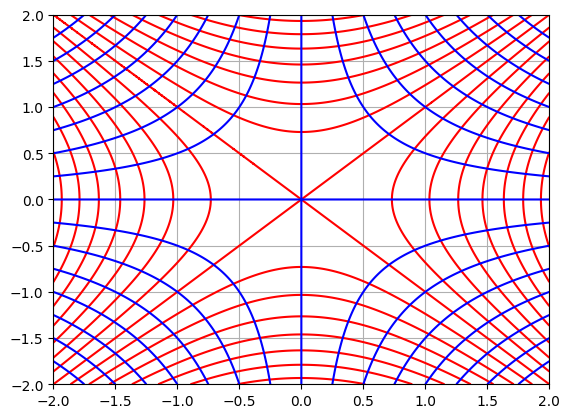
\includegraphics[width=0.35\textwidth]{pictures/funcio_exemple_corbes_nivell.png}
        \begin{adjustwidth}{1cm}{1cm}
            \caption{Corbes de nivell de $f(z)=\frac{3}{2}z^2$: en roig les que fixen $u(z)$ i en blau les que fixen $v(z)$.}
        \end{adjustwidth}
        \label{Corbes_nivell_exemple} 
    \end{figure}
    
    \end{subsection}

\end{adjustwidth}